\documentclass{standalone}
\usepackage{tikz}
\usetikzlibrary{patterns, positioning}


\begin{document}
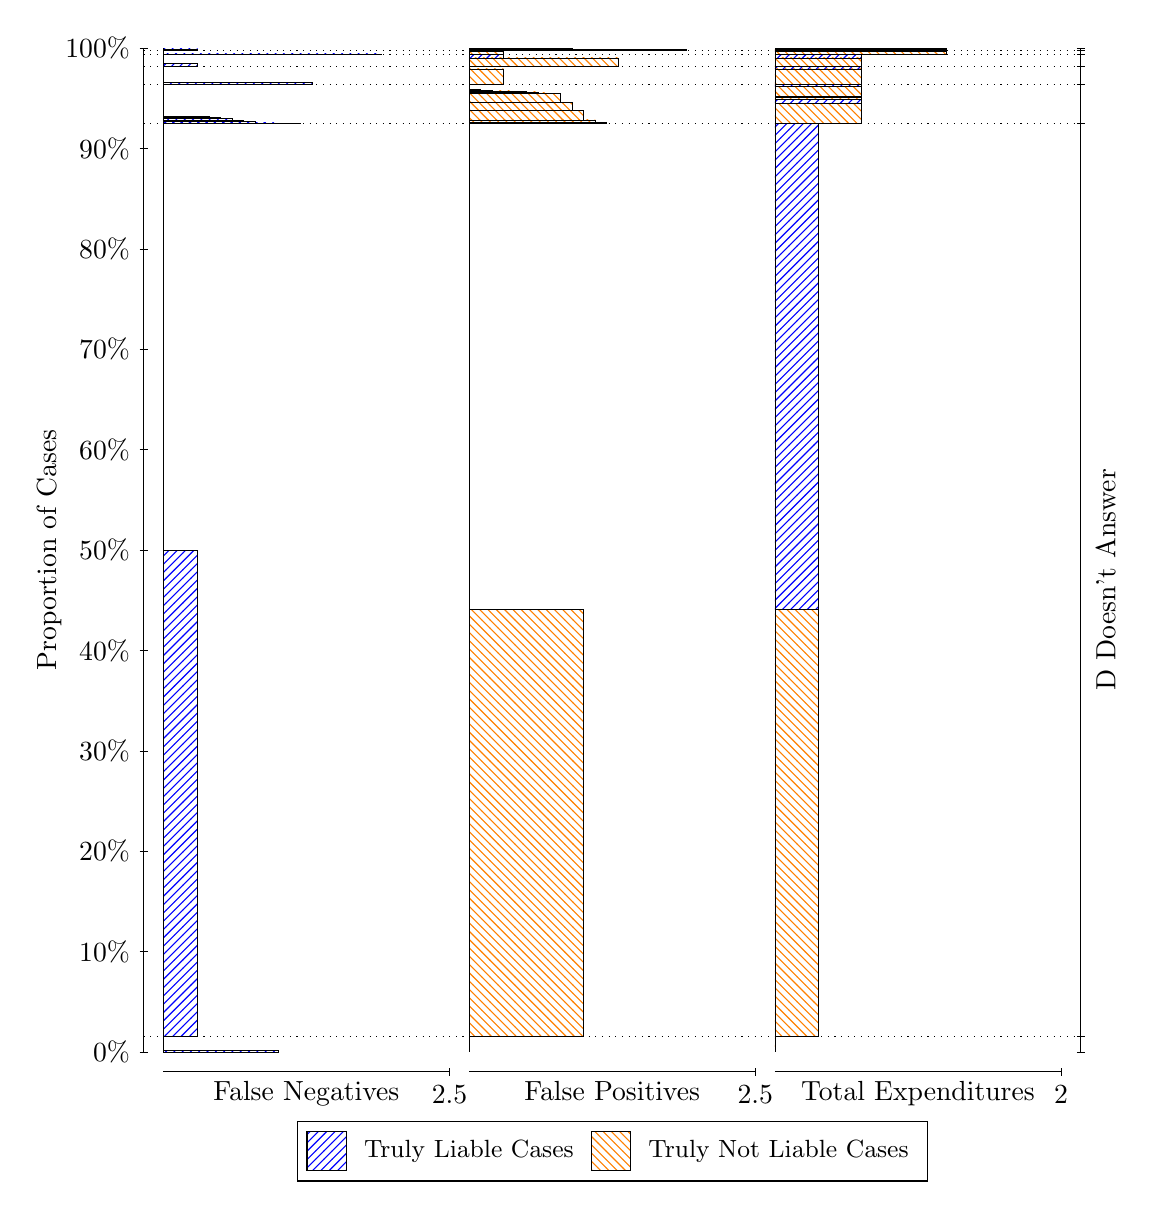
\begin{tikzpicture}
\draw[black, very thin] (1.5,1.75) -- (1.5,14.5);
\node[rotate=90, text=black, anchor=center] at (0.3, 8.125) {Proportion of Cases};
\draw[black, very thin] (1.45,1.75) -- (1.55,1.75);
\node[text=black, anchor=east] at (1.45, 1.75) {0\%};
\draw[black, very thin] (1.45,3.025) -- (1.55,3.025);
\node[text=black, anchor=east] at (1.45, 3.025) {10\%};
\draw[black, very thin] (1.45,4.3) -- (1.55,4.3);
\node[text=black, anchor=east] at (1.45, 4.3) {20\%};
\draw[black, very thin] (1.45,5.575) -- (1.55,5.575);
\node[text=black, anchor=east] at (1.45, 5.575) {30\%};
\draw[black, very thin] (1.45,6.85) -- (1.55,6.85);
\node[text=black, anchor=east] at (1.45, 6.85) {40\%};
\draw[black, very thin] (1.45,8.125) -- (1.55,8.125);
\node[text=black, anchor=east] at (1.45, 8.125) {50\%};
\draw[black, very thin] (1.45,9.4) -- (1.55,9.4);
\node[text=black, anchor=east] at (1.45, 9.4) {60\%};
\draw[black, very thin] (1.45,10.675) -- (1.55,10.675);
\node[text=black, anchor=east] at (1.45, 10.675) {70\%};
\draw[black, very thin] (1.45,11.95) -- (1.55,11.95);
\node[text=black, anchor=east] at (1.45, 11.95) {80\%};
\draw[black, very thin] (1.45,13.225) -- (1.55,13.225);
\node[text=black, anchor=east] at (1.45, 13.225) {90\%};
\draw[black, very thin] (1.45,14.5) -- (1.55,14.5);
\node[text=black, anchor=east] at (1.45, 14.5) {100\%};

\draw[black, very thin] (13.4,1.75) -- (13.4,14.5);
\draw[black, very thin] (13.35,1.75) -- (13.45,1.75);
\node[anchor=west] at (13.35, 1.75) {};
\draw[black, very thin] (13.35,1.9465) -- (13.45,1.9465);
\node[anchor=west] at (13.35, 1.9465) {};
\draw[black, very thin] (13.35,13.543) -- (13.45,13.543);
\node[anchor=west] at (13.35, 13.543) {};
\draw[black, very thin] (13.35,14.039) -- (13.45,14.039);
\node[anchor=west] at (13.35, 14.039) {};
\draw[black, very thin] (13.35,14.263) -- (13.45,14.263);
\node[anchor=west] at (13.35, 14.263) {};
\draw[black, very thin] (13.35,14.415) -- (13.45,14.415);
\node[anchor=west] at (13.35, 14.415) {};
\draw[black, very thin] (13.35,14.473) -- (13.45,14.473);
\node[anchor=west] at (13.35, 14.473) {};
\draw[black, very thin] (13.35,14.5) -- (13.45,14.5);
\node[anchor=west] at (13.35, 14.5) {};

\draw[black, very thin, pattern color=blue, pattern=north east lines] (1.75,1.75) rectangle (3.2033,1.7707);
\draw[black, very thin, pattern color=orange, pattern=north west lines] (1.75,1.7707) rectangle (1.75,1.9465);
\draw[black, very thin, pattern color=blue, pattern=north east lines] (1.75,1.9465) rectangle (2.186,8.1205);
\draw[black, very thin, pattern color=orange, pattern=north west lines] (1.75,8.1205) rectangle (1.75,13.543);
\draw[black, very thin, pattern color=blue, pattern=north east lines] (1.75,13.543) rectangle (3.494,13.544);
\draw[black, very thin, pattern color=blue, pattern=north east lines] (1.75,13.544) rectangle (3.3487,13.545);
\draw[black, very thin, pattern color=blue, pattern=north east lines] (1.75,13.545) rectangle (3.2033,13.548);
\draw[black, very thin, pattern color=blue, pattern=north east lines] (1.75,13.548) rectangle (3.058,13.549);
\draw[black, very thin, pattern color=blue, pattern=north east lines] (1.75,13.549) rectangle (3.058,13.55);
\draw[black, very thin, pattern color=blue, pattern=north east lines] (1.75,13.55) rectangle (2.9127,13.568);
\draw[black, very thin, pattern color=blue, pattern=north east lines] (1.75,13.568) rectangle (2.7673,13.585);
\draw[black, very thin, pattern color=blue, pattern=north east lines] (1.75,13.585) rectangle (2.622,13.61);
\draw[black, very thin, pattern color=blue, pattern=north east lines] (1.75,13.61) rectangle (2.4767,13.62);
\draw[black, very thin, pattern color=blue, pattern=north east lines] (1.75,13.62) rectangle (2.3313,13.627);
\draw[black, very thin, pattern color=orange, pattern=north west lines] (1.75,13.627) rectangle (1.75,14.039);
\draw[black, very thin, pattern color=blue, pattern=north east lines] (1.75,14.039) rectangle (3.6393,14.068);
\draw[black, very thin, pattern color=orange, pattern=north west lines] (1.75,14.068) rectangle (1.75,14.263);
\draw[black, very thin, pattern color=blue, pattern=north east lines] (1.75,14.263) rectangle (2.186,14.303);
\draw[black, very thin, pattern color=orange, pattern=north west lines] (1.75,14.303) rectangle (1.75,14.415);
\draw[black, very thin, pattern color=blue, pattern=north east lines] (1.75,14.415) rectangle (4.5113,14.426);
\draw[black, very thin, pattern color=orange, pattern=north west lines] (1.75,14.426) rectangle (1.75,14.473);
\draw[black, very thin, pattern color=blue, pattern=north east lines] (1.75,14.473) rectangle (2.186,14.489);
\draw[black, very thin, pattern color=orange, pattern=north west lines] (1.75,14.489) rectangle (1.75,14.5);
\draw[black, very thin, pattern color=orange, pattern=north west lines] (5.6333,1.75) rectangle (5.6333,1.9259);
\draw[black, very thin, pattern color=blue, pattern=north east lines] (5.6333,1.9259) rectangle (5.6333,1.9465);
\draw[black, very thin, pattern color=orange, pattern=north west lines] (5.6333,1.9465) rectangle (7.0867,7.369);
\draw[black, very thin, pattern color=blue, pattern=north east lines] (5.6333,7.369) rectangle (5.6333,13.543);
\draw[black, very thin, pattern color=orange, pattern=north west lines] (5.6333,13.543) rectangle (7.3773,13.558);
\draw[black, very thin, pattern color=orange, pattern=north west lines] (5.6333,13.558) rectangle (7.232,13.587);
\draw[black, very thin, pattern color=orange, pattern=north west lines] (5.6333,13.587) rectangle (7.0867,13.705);
\draw[black, very thin, pattern color=orange, pattern=north west lines] (5.6333,13.705) rectangle (6.9413,13.814);
\draw[black, very thin, pattern color=orange, pattern=north west lines] (5.6333,13.814) rectangle (6.796,13.919);
\draw[black, very thin, pattern color=orange, pattern=north west lines] (5.6333,13.919) rectangle (6.6507,13.931);
\draw[black, very thin, pattern color=orange, pattern=north west lines] (5.6333,13.931) rectangle (6.5053,13.943);
\draw[black, very thin, pattern color=orange, pattern=north west lines] (5.6333,13.943) rectangle (6.36,13.949);
\draw[black, very thin, pattern color=orange, pattern=north west lines] (5.6333,13.949) rectangle (6.2147,13.955);
\draw[black, very thin, pattern color=blue, pattern=north east lines] (5.6333,13.955) rectangle (5.924,13.962);
\draw[black, very thin, pattern color=blue, pattern=north east lines] (5.6333,13.962) rectangle (5.7787,13.972);
\draw[black, very thin, pattern color=blue, pattern=north east lines] (5.6333,13.972) rectangle (5.6333,14.039);
\draw[black, very thin, pattern color=orange, pattern=north west lines] (5.6333,14.039) rectangle (6.0693,14.234);
\draw[black, very thin, pattern color=blue, pattern=north east lines] (5.6333,14.234) rectangle (5.6333,14.263);
\draw[black, very thin, pattern color=orange, pattern=north west lines] (5.6333,14.263) rectangle (7.5227,14.375);
\draw[black, very thin, pattern color=blue, pattern=north east lines] (5.6333,14.375) rectangle (6.0693,14.415);
\draw[black, very thin, pattern color=orange, pattern=north west lines] (5.6333,14.415) rectangle (6.0693,14.462);
\draw[black, very thin, pattern color=blue, pattern=north east lines] (5.6333,14.462) rectangle (5.6333,14.473);
\draw[black, very thin, pattern color=orange, pattern=north west lines] (5.6333,14.473) rectangle (8.3947,14.484);
\draw[black, very thin, pattern color=blue, pattern=north east lines] (5.6333,14.484) rectangle (6.9413,14.5);
\draw[black, very thin, pattern color=orange, pattern=north west lines] (9.5167,1.75) rectangle (9.5167,1.9259);
\draw[black, very thin, pattern color=blue, pattern=north east lines] (9.5167,1.9259) rectangle (9.5167,1.9465);
\draw[black, very thin, pattern color=orange, pattern=north west lines] (9.5167,1.9465) rectangle (10.062,7.369);
\draw[black, very thin, pattern color=blue, pattern=north east lines] (9.5167,7.369) rectangle (10.062,13.543);
\draw[black, very thin, pattern color=orange, pattern=north west lines] (9.5167,13.543) rectangle (10.607,13.795);
\draw[black, very thin, pattern color=blue, pattern=north east lines] (9.5167,13.795) rectangle (10.607,13.848);
\draw[black, very thin, pattern color=orange, pattern=north west lines] (9.5167,13.848) rectangle (10.607,13.877);
\draw[black, very thin, pattern color=blue, pattern=north east lines] (9.5167,13.877) rectangle (10.607,13.884);
\draw[black, very thin, pattern color=orange, pattern=north west lines] (9.5167,13.884) rectangle (10.607,14.013);
\draw[black, very thin, pattern color=blue, pattern=north east lines] (9.5167,14.013) rectangle (10.607,14.039);
\draw[black, very thin, pattern color=orange, pattern=north west lines] (9.5167,14.039) rectangle (10.607,14.234);
\draw[black, very thin, pattern color=blue, pattern=north east lines] (9.5167,14.234) rectangle (10.607,14.263);
\draw[black, very thin, pattern color=orange, pattern=north west lines] (9.5167,14.263) rectangle (10.607,14.375);
\draw[black, very thin, pattern color=blue, pattern=north east lines] (9.5167,14.375) rectangle (10.607,14.415);
\draw[black, very thin, pattern color=orange, pattern=north west lines] (9.5167,14.415) rectangle (11.697,14.462);
\draw[black, very thin, pattern color=blue, pattern=north east lines] (9.5167,14.462) rectangle (11.697,14.473);
\draw[black, very thin, pattern color=orange, pattern=north west lines] (9.5167,14.473) rectangle (11.697,14.484);
\draw[black, very thin, pattern color=blue, pattern=north east lines] (9.5167,14.484) rectangle (11.697,14.5);
\draw[black, dotted] (1.5,1.9465) -- (13.4,1.9465);
\draw[black, dotted] (1.5,13.543) -- (13.4,13.543);
\draw[black, dotted] (1.5,14.039) -- (13.4,14.039);
\draw[black, dotted] (1.5,14.263) -- (13.4,14.263);
\draw[black, dotted] (1.5,14.415) -- (13.4,14.415);
\draw[black, dotted] (1.5,14.473) -- (13.4,14.473);
\draw[black, very thin] (1.75,1.5) -- (5.3833,1.5);
\node[text=black, anchor=north] at (3.5667, 1.5) {False Negatives};
\draw[black, very thin] (5.3833,1.45) -- (5.3833,1.55);
\node[text=black, anchor=north] at (5.3833, 1.45) {2.5};

\draw[black, very thin] (5.6333,1.5) -- (9.2667,1.5);
\node[text=black, anchor=north] at (7.45, 1.5) {False Positives};
\draw[black, very thin] (9.2667,1.45) -- (9.2667,1.55);
\node[text=black, anchor=north] at (9.2667, 1.45) {2.5};

\draw[black, very thin] (9.5167,1.5) -- (13.15,1.5);
\node[text=black, anchor=north] at (11.333, 1.5) {Total Expenditures};
\draw[black, very thin] (13.15,1.45) -- (13.15,1.55);
\node[text=black, anchor=north] at (13.15, 1.45) {2};


\node[text=black, centered, rotate=90] at (13.72, 7.7447) {D Doesn't Answer};






\draw (7.449999999999999,1.5) node[draw=none] (baseCoordinate) {};
\begin{scope}[align=center]
        \matrix[scale=0.5, draw=black, below=0.5cm of baseCoordinate, nodes={draw}, column sep=0.1cm]{
            \node[rectangle, draw, minimum width=0.5cm, minimum height=0.5cm, pattern color=blue, pattern=north east lines] {}; &
            \node[draw=none, font=\small, text=black] (B) {Truly Liable Cases}; &
            \node[rectangle, draw, minimum width=0.5cm, minimum height=0.5cm, pattern color=orange, pattern=north west lines] {}; &
            \node[draw=none, font=\small, text=black] (B) {Truly Not Liable Cases}; \\
            };
\end{scope}

\end{tikzpicture}
\end{document}